\documentclass[10pt]{article}
\usepackage[polish]{babel}
\usepackage[utf8]{inputenc}
\usepackage[T1]{fontenc}
\usepackage{amsmath}
\usepackage{amsfonts}
\usepackage{amssymb}
\usepackage[version=4]{mhchem}
\usepackage{stmaryrd}
\usepackage{graphicx}
\usepackage[export]{adjustbox}
\graphicspath{ {./images/} }

\title{LIGA MATEMATYCZNA \\
 im. Zdzisława Matuskiego \\
 GRUDZIEŃ 2022 \\
 SZKOŁA PODSTAWOWA \\
 klasy VII - VIII }

\author{}
\date{}


\begin{document}
\maketitle
\section*{ZADANIE 1.}
Ile dzielników ma liczba \(2^{2} \cdot 3^{5}+2 \cdot 3^{6}+2^{3} \cdot 3^{7}\) ?

\section*{ZADANIE 2.}
Na prostej zawierającej wysokość \(B D\) trójkąta równobocznego \(A B C\) wybrano punkt \(K\) tak, aby \(|B K|=|A C|\). Punkt \(K\) połączono z punktami \(A\) i \(C\). Oblicz miarę kąta \(A K C\).

\section*{ZADANIE 3.}
Czy liczbę 55555553 można przedstawić w postaci sumy dwóch liczb pierwszych?

\section*{ZADANIE 4.}
Suma cyfr pewnej nieparzystej liczby trzycyfrowej podzielnej przez pięć jest trzy razy większa niż cyfra jedności. Suma cyfr jedności i setek jest cztery razy większa niż cyfra dziesiątek. Znajdź tę liczbę.

\section*{ZADANIE 5.}
Duży trójkąt podzielono na mniejsze trójkąty tak, jak na rysunku. Liczby wewnątrz małych trójkątów oznaczają ich obwody. Oblicz obwód dużego trójkąta.\\
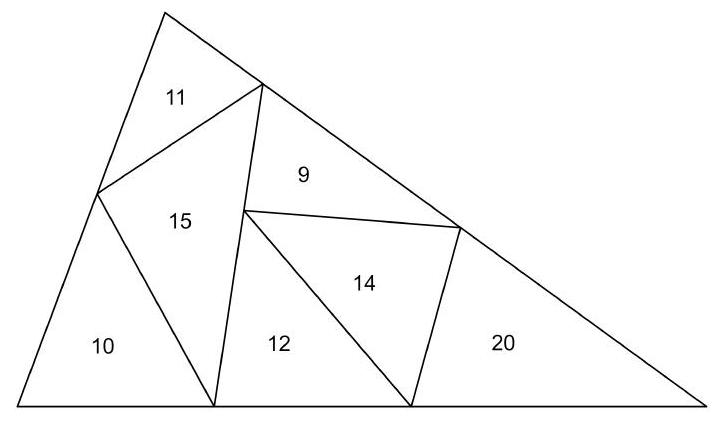
\includegraphics[max width=\textwidth, center]{2024_11_21_fdad45e33c34501d05e2g-1}


\end{document}